% In this chapter we have reviewed differentiation. We've defined the derivative as the instantaneous rate of change of a function, and looked at estimating derivatives using tables and graphs. We've reviewed the formulas for derivatives of basic functions, as well as the product, quotient, and chain rules. We've looked at derivatives of implicitly defined functions and inverse functions, and reviewed two important theorems: Rolle's Theorem and the Mean Value Theorem.
% 
% For BC Calculus students, we've reviewed derivatives of parametrically defined functions and the use of L'Hopital's Rule for evaluating limits of indeterminate forms.
% 
\begin{EnvFullwidth}
\textit{In each of Questions~\ref{calc03:deriv-first}--\ref{calc03:deriv-last}, a function is given. Choose the alternative that is the derivative $\dfrac{d y}{d x}$ of the function.}
\end{EnvFullwidth} 

\question\label{calc03:deriv-first}
$y=x^{5} \tan x$
\begin{choices}
  \choice $5 x^{4} \tan x$
  \choice $x^{5} \sec ^{2} x$
  \choice $5 x^{4} \sec ^{2} x$
  \choice $5 x^{4}+\sec ^{2} x$
  \CorrectChoice $5 x^{4} \tan x+x^{5} \sec ^{2} x$
\end{choices}
\begin{solution}
By the Product Rule, (5),


\[
y^{\prime}=x^{5}(\tan x)^{\prime}+\left(x^{5}\right)^{\prime}(\tan x) .
\]


\end{solution}

\question
$y=\dfrac{2-x}{3 x+1}$
\begin{choices}
  \CorrectChoice $-\dfrac{7}{(3 x+1)^{2}}$
  \choice $\dfrac{6 x-5}{(3 x+1)^{2}}$
  \choice $-\dfrac{9}{(3 x+1)^{2}}$
  \choice $\dfrac{7}{(3 x+1)^{2}}$
  \choice $\dfrac{7-6 x}{(3 x+1)^{2}}$
\end{choices}
\begin{solution}
By the Quotient Rule, (6),
\[
y^{\prime}=\dfrac{(3 x+1)(-1)-(2-x)(3)}{(3 x+1)^{2}}=-\dfrac{7}{(3 x+1)^{2}} .
\]
\end{solution}


\newpage


\question
$y=\sqrt{3-2 x}$
\begin{choices}
  \choice $\dfrac{1}{2 \sqrt{3-2 x}}$
  \CorrectChoice $-\dfrac{1}{\sqrt{3-2 x}}$
  \choice $-\dfrac{(3-2 x)^{3 / 2}}{3}$
  \choice $-\dfrac{1}{3-2 x}$
  \choice $\dfrac{2}{3}(3-2 x)^{3 / 2}$
\end{choices}
\begin{solution}
Since $y=(3-2 x)^{1 / 2}$, by the Power Rule, (3),


\[
y^{\prime}=\dfrac{1}{2}(3-3 x)^{-1 / 2} \cdot(-2)=-\dfrac{1}{\sqrt{3-2 x}} .
\]


\end{solution}

\question
$y=\dfrac{2}{(5 x+1)^{3}}$
\begin{choices}
  \choice $-\dfrac{30}{(5 x+1)^{2}}$
  \CorrectChoice $-30(5 x+1)^{-4}$
  \choice $\dfrac{-6}{(5 x+1)^{4}}$
  \choice $-\dfrac{10}{3}(5 x+1)^{-4 / 3}$
  \choice $\dfrac{30}{(5 x+1)^{4}}$
\end{choices}
\begin{solution}
Since $y=2(5 x+1)^{-3}, y^{\prime}=-6(5 x+1)^{-4}(5)$.
\end{solution}

\question
$y=3 x^{2 / 3}-4 x^{1 / 2}-2$
\begin{choices}
  \choice $2 x^{1 / 3}-2 x^{-1 / 2}$
  \choice $3 x^{-1 / 3}-2 x^{-1 / 2}$
  \choice $\dfrac{9}{5} x^{5 / 3}-8 x^{3 / 2}$
  \choice $\dfrac{2}{x^{1 / 3}}-\dfrac{2}{x^{1 / 2}}-2$
  \CorrectChoice $2 x^{-1 / 3}-2 x^{-1 / 2}$
\end{choices}
\begin{solution}
$y^{\prime}=3\left(\dfrac{2}{3}\right) x^{-1 / 3}-4\left(\dfrac{1}{2}\right) x^{-1 / 2}$
\end{solution}


\newpage


\question
$y=2 \sqrt{x}-\dfrac{1}{2 \sqrt{x}}$
\begin{choices}
  \choice $x+\dfrac{1}{x \sqrt{x}}$
  \choice $x^{-1 / 2}+x^{-3 / 2}$
  \choice $\dfrac{4 x-1}{4 x \sqrt{x}}$
  \CorrectChoice $\dfrac{1}{\sqrt{x}}+\dfrac{1}{4 x \sqrt{x}}$
  \choice $\dfrac{4}{\sqrt{x}}+\dfrac{1}{x \sqrt{x}}$
\end{choices}
\begin{solution}
Rewrite: $y=2 x^{1 / 2}-\dfrac{1}{2} x^{1 / 2}$, so $y^{\prime}=x^{-1 / 2}+\dfrac{1}{4} x^{-3 / 2}$.
\end{solution}

\question
$y=\sqrt{x^{2}+2 x-1}$
\begin{choices}
  \CorrectChoice $\dfrac{x+1}{y}$
  \choice $4 y(x+1)$
  \choice $\dfrac{1}{2 \sqrt{x^{2}+2 x-1}}$
  \choice $-\dfrac{x+1}{\left(x^{2}+2 x-1\right)^{3 / 2}}$
  \choice none of these
\end{choices}
\begin{solution}
Rewrite: $y=\left(x^{2}+2 x-1\right)^{1 / 2}$; then $y=\dfrac{1}{2}\left(x^{2}+2 x-1\right)^{-1 / 2}(2 x+2)$
\end{solution}

\question
$y=\dfrac{x^{2}}{\cos x}$
\begin{choices}
  \choice $\dfrac{2 x}{\sin x}$
  \choice $-\dfrac{2 x}{\sin x}$
  \choice $\dfrac{2 x \cos x-x^{2} \sin x}{\cos ^{2} x}$
  \CorrectChoice $\dfrac{2 x \cos x+x^{2} \sin x}{\cos ^{2} x}$
  \choice $\dfrac{2 x \cos x+x^{2} \sin x}{\sin ^{2} x}$
\end{choices}
\begin{solution}
Use the Quotient Rule:
\[
y^{\prime}=\dfrac{2 x \cos x-x^{2}(-\sin x)}{\cos ^{2} x}
\]
\end{solution}


\newpage


\question
$y=\ln \dfrac{e^{x}}{e^{x}-1}$
\begin{choices}
  \choice $x-\dfrac{e^{x}}{e^{x}-1}$
  \choice $\dfrac{1}{e^{x}-1}$
  \CorrectChoice $-\dfrac{1}{e^{x}-1}$
  \choice $0$
  \choice $\dfrac{e^{x}-2}{e^{x}-1}$
\end{choices}
\begin{solution}
Since


\[
\begin{aligned}
y & =\ln e^{x}-\ln \left(e^{x}-1\right) \\
& =x-\ln \left(e^{x}-1\right)
\end{aligned}
\]
then
\[
y^{\prime}=1-\dfrac{e^{x}}{e^{x}-1}=\dfrac{e^{x}-1-e^{x}}{e^{x}-1}=-\dfrac{1}{e^{x}-1}
\]
\end{solution}

\question
$y=\tan ^{-1} \dfrac{x}{2}$
\begin{choices}
  \choice $\dfrac{4}{4+x^{2}}$
  \choice $\dfrac{1}{2 \sqrt{4-x^{2}}}$
  \choice $\dfrac{2}{\sqrt{4-x^{2}}}$
  \choice $\dfrac{1}{2+x^{2}}$
  \CorrectChoice $\dfrac{2}{x^{2}+4}$
\end{choices}
\begin{solution}
Use formula (18): $y^{\prime}=\dfrac{\dfrac{1}{2}}{1+\dfrac{x^{2}}{4}}$.
\end{solution}


\newpage


\question
$y=\ln (\sec x+\tan x)$
\begin{choices}
  \CorrectChoice $\sec x$
  \choice $\dfrac{1}{\sec x}$
  \choice $\tan x+\dfrac{\sec ^{2} x}{\tan x}$
  \choice $\dfrac{1}{\sec x+\tan x}$
  \choice $-\dfrac{1}{\sec x+\tan x}$
\end{choices}
\begin{solution}
Use formulas (13), (11), and (9):


\[
y^{\prime}=\dfrac{\sec x \tan x+\sec ^{2} x}{\sec x+\tan x}=\dfrac{\sec x(\tan x+\sec x)}{\sec x+\tan x} .
\]


\end{solution}

\question
$y=\dfrac{e^{x}-e^{-x}}{e^{x}+e^{-x}}$
\begin{choices}
  \choice $0$
  \choice $1$
  \choice $\dfrac{2}{\left(e^{x}+e^{-x}\right)^{2}}$
  \CorrectChoice $\dfrac{4}{\left(e^{x}+e^{-x}\right)^{2}}$
  \choice $\dfrac{1}{e^{2 x}+e^{-2 x}}$
\end{choices}
\begin{solution}
By the Quotient Rule,
\[
\begin{aligned}
y^{\prime} & =\dfrac{\left(e^{x}+e^{-x}\right)\left(e^{x}+e^{-x}\right)-\left(e^{x}-e^{-x}\right)\left(e^{x}-e^{-x}\right)}{\left(e^{x}+e^{-x}\right)^{2}} \\
& =\dfrac{\left(e^{2 x}+2+e^{-2 x}\right)-\left(e^{2 x}-2+e^{-2 x}\right)}{\left(e^{x}+e^{-x}\right)^{2}}=\dfrac{4}{\left(e^{x}+e^{-x}\right)^{2}} .
\end{aligned}
\]
\end{solution}


\newpage


\question
$y=\ln \left(\sqrt{x^{2}+1}\right)$
\begin{choices}
  \choice $\dfrac{1}{\sqrt{x^{2}+1}}$
  \choice $\dfrac{2 x}{\sqrt{x^{2}+1}}$
  \choice $\dfrac{1}{2\left(x^{2}+1\right)}$
  \CorrectChoice $\dfrac{x}{x^{2}+1}$
  \choice $\dfrac{2 x}{x^{2}+1}$
\end{choices}
\begin{solution}
Since $y=\dfrac{1}{2} \ln \left(x^{2}+1\right)$,


\[
y^{\prime}=\dfrac{1}{2} \cdot \dfrac{2 x}{x^{2}+1} .
\]


\end{solution}

\question
$y=\sin \left(\dfrac{1}{x}\right)$
\begin{choices}
  \choice $\cos \left(\dfrac{1}{x}\right)$
  \choice $\cos \left(-\dfrac{1}{x^{2}}\right)$
  \CorrectChoice $-\dfrac{1}{x^{2}} \cos \left(\dfrac{1}{x}\right)$
  \choice $-\dfrac{1}{x^{2}} \sin \left(\dfrac{1}{x}\right)+\dfrac{1}{x} \cos \left(\dfrac{1}{x}\right)$
  \choice $\cos (\ln x)$
\end{choices}
\begin{solution}
$y^{\prime}=\sin ^{\prime}\left(\dfrac{1}{x}\right) \cdot\left(\dfrac{1}{x}\right)^{\prime}=\cos \left(\dfrac{1}{x}\right) \cdot\left(-\dfrac{1}{x^{2}}\right)$
\end{solution}

\question
$y=\dfrac{1}{2 \sin 2 x}$
\begin{choices}
  \CorrectChoice $-\csc 2 x \cot 2 x$
  \choice $\dfrac{1}{4 \cos 2 x}$
  \choice $-4 \csc 2 x \cot 2 x$
  \choice $\dfrac{\cos 2 x}{2 \sqrt{\sin 2 x}}$
  \choice $-\csc ^{2} 2 x$
\end{choices}
\begin{solution}
Since $y=\dfrac{1}{2} \csc 2 x, y^{\prime}=\dfrac{1}{2}(-\csc 2 x \cot 2 x \cdot 2)$.
\end{solution}


\newpage


\question
$y=e^{-x} \cos 2 x$
\begin{choices}
  \CorrectChoice $-e^{-x}(\cos 2 x+2 \sin 2 x)$
  \choice $e^{-x}(\sin 2 x-\cos 2 x)$
  \choice $2 e^{-x} \sin 2 x$
  \choice $-e^{-x}(\cos 2 x+\sin 2 x)$
  \choice $-e^{-x} \sin 2 x$
\end{choices}
\begin{solution}
$y^{\prime}=e^{-x}(-2 \sin 2 x)+\cos 2 x\left(-e^{-x}\right)$.
\end{solution}

\question
$y=\sec ^{2}(x)$
\begin{choices}
  \choice $2 \sec x$
  \choice $2 \sec x \tan x$
  \CorrectChoice $2 \sec ^{2} x \tan x$
  \choice $\sec ^{2} x \tan ^{2} x$
  \choice $\tan x$
\end{choices}
\begin{solution}
$y^{\prime}=(2 \sec x)(\sec x \tan x)$
\end{solution}

\question
$y=x \ln ^{3} x$
\begin{choices}
  \choice $\dfrac{3 \ln ^{2} x}{x}$
  \choice $3 \ln ^{2} x$
  \choice $3 x \ln ^{2} x+\ln ^{3} x$
  \choice $3(\ln x+1)$
  \CorrectChoice none of these
\end{choices}
\begin{solution}
$y^{\prime}=\dfrac{x\left(3 \ln ^{2} x\right)}{x}+\ln ^{3} x$. The correct answer is $3 \ln ^{2} x+\ln ^{3} x$.
\end{solution}



\newpage



\question
$y=\dfrac{1+x^{2}}{1-x^{2}}$
\begin{choices}
  \choice $-\dfrac{4 x}{\left(1-x^{2}\right)^{2}}$
  \CorrectChoice $\dfrac{4 x}{\left(1-x^{2}\right)^{2}}$
  \choice $\dfrac{-4 x^{3}}{\left(1-x^{2}\right)^{2}}$
  \choice $\dfrac{2 x}{1-x^{2}}$
  \choice $\dfrac{4}{1-x^{2}}$
\end{choices}
\begin{solution}
$y^{\prime}=\dfrac{\left(1-x^{2}\right)(2 x)-\left(1+x^{2}\right)(-2 x)}{\left(1-x^{2}\right)^{2}}$.
\end{solution}

\question\label{calc03:deriv-last}
$y=\sin ^{-1} x-\sqrt{1-x^{2}}$
\begin{choices}
  \choice $\dfrac{1}{2 \sqrt{1-x^{2}}}$
  \choice $\dfrac{2}{\sqrt{1-x^{2}}}$
  \CorrectChoice $\dfrac{1+x}{\sqrt{1-x^{2}}}$
  \choice $\dfrac{x^{2}}{\sqrt{1-x^{2}}}$
  \choice $\dfrac{1}{\sqrt{1+x}}$
\end{choices}
\begin{solution}
$y^{\prime}=\dfrac{1}{\sqrt{1-x^{2}}}-\dfrac{1 \cdot(-2 x)}{2 \sqrt{1-x^{2}}}$.
\end{solution}




\newpage



\begin{EnvFullwidth}
\textit{In each of Questions~\ref{calc03:implicit-first}--\ref{calc03:implicit-last}, $y$ is a differentiable function of $x$. Choose the alternative that is the derivative $\dfrac{d y}{d x}$.}
\end{EnvFullwidth}

\question\label{calc03:implicit-first}
$x^{3}-y^{3}=1$
\begin{choices}
  \choice $x$
  \choice $3 x^{2}$
  \choice $\sqrt[3]{3 x^{2}}$
  \CorrectChoice $\dfrac{x^{2}}{y^{2}}$
  \choice $\dfrac{3 x^{2}-1}{y^{2}}$
\end{choices}
\begin{solution}
Let $y^{\prime}$ be $\dfrac{d y}{d x}$; then $3 x^{2}-3 y^{2} y^{\prime}=0 ; y^{\prime}=\dfrac{-3 x^{2}}{-3 y^{2}}$.
\end{solution}

\question
$x+\cos (x+y)=0$
\begin{choices}
  \CorrectChoice $\csc (x+y)-1$
  \choice $\csc (x+y)$
  \choice $\dfrac{x}{\sin (x+y)}$
  \choice $\dfrac{1}{\sqrt{1-x^{2}}}$
  \choice $\dfrac{1-\sin x}{\sin y}$
\end{choices}
\begin{solution}
$1-\sin (x+y)\left(1+y^{\prime}\right)=0 ; \dfrac{1-\sin (x+y)}{\sin (x+y)}=y^{\prime}$.
\end{solution}

\question
$\sin x-\cos y-2=0$
\begin{choices}
  \choice $-\cot x$
  \choice $-\cot y$
  \choice $\dfrac{\cos x}{\sin y}$
  \CorrectChoice $-\csc y \cos x$
  \choice $\dfrac{2-\cos x}{\sin y}$
\end{choices}
\begin{solution}
$\cos x+\sin y \cdot y^{\prime}=0 ; y^{\prime}=-\dfrac{\cos x}{\sin y}$.
\end{solution}




\newpage



\question\label{calc03:implicit-last}
$3 x^{2}-2 x y+5 y^{2}=1$
\begin{choices}
  \choice $\dfrac{3 x+y}{x-5 y}$
  \CorrectChoice $\dfrac{y-3 x}{5 y-x}$
  \choice $3 x+5 y$
  \choice $\dfrac{3 x+4 y}{x}$
  \choice none of these
\end{choices}
\begin{solution}
$6 x-2\left(x y^{\prime}+y\right)+10 y y^{\prime}=0 ; y^{\prime}(10 y-2 x)=2 y-6 x$.
\end{solution}

\question
If $x=t^{2}+1$ and $y=2 t^{3}$, then $\dfrac{d y}{d x}=$
\begin{choices}
  \CorrectChoice $3 t$
  \choice $6 t^{2}$
  \choice $\dfrac{6 t^{2}}{t^{2}+1}$
  \choice $\dfrac{6 t^{2}}{\left(t^{2}+1\right)^{2}}$
  \choice $\dfrac{2 t^{4}+6 t^{2}}{\left(t^{2}+1\right)^{2}}$
\end{choices}
\begin{solution}
$\dfrac{d y}{d x}=\dfrac{d y / d t}{d x / d t}=\dfrac{6 t^{2}}{2 t}$
\end{solution}

\question
If $f(x)=x^{4}-4 x^{3}+4 x^{2}-1$, then the set of values of $x$ for which the derivative equals zero is
\begin{choices}
  \choice $\{1,2\}$
  \choice $\{0,-1,-2\}$
  \choice $\{-1,+2\}$
  \choice $\{0\}$
  \CorrectChoice $\{0,1,2\}$
\end{choices}
\begin{solution}
$f^{\prime}(x)=4 x^{3}-12 x^{2}+8 x=4 x(x-1)(x-2)$.
\end{solution}




\newpage



\question
If $f(x)=16 \sqrt{x}$, then $f^{\prime \prime}(4)$ is equal to
\begin{choices}
  \choice $-32$
  \choice $-16$
  \choice $-4$
  \choice $-2$
  \CorrectChoice $-\dfrac{1}{2}$
\end{choices}
\begin{solution}
$f^{\prime}(x)=8 x^{-1 / 2} ; f^{\prime \prime}(x)=-4 x^{-3 / 2}=-\dfrac{4}{x^{3 / 2}} ; f^{\prime \prime}(4)=-\dfrac{4}{8}$.
\end{solution}

\question
If $f(x)=\ln x^{3}$, then $f^{\prime \prime}(3)$ is
\begin{choices}
  \CorrectChoice $-\dfrac{1}{3}$
  \choice $-1$
  \choice $-3$
  \choice $1$
  \choice none of these
\end{choices}
\begin{solution}
$f(x)=3 \ln x ; f^{\prime}(x)=\dfrac{3}{x} ; f^{\prime \prime}(x)=\dfrac{-3}{x^{2}}$. Replace $x$ by 3 .
\end{solution}

\question
If a point moves on the curve $x^{2}+y^{2}=25$, then, at $(0,5), \dfrac{d^{2} y}{d x^{2}}$ is
\begin{choices}
  \choice $0$
  \choice $\dfrac{1}{5}$
  \choice $-5$
  \CorrectChoice $-\dfrac{1}{5}$
  \choice nonexistent
\end{choices}
\begin{solution}
$2 x+2 y y^{\prime}=0 ; y^{\prime}=-\dfrac{x}{y} ; y^{\prime \prime}=-\dfrac{y-x y^{\prime}}{y^{2}}$. At $(0,5), y^{\prime \prime}=-\dfrac{5-0}{25}$.
\end{solution}




\newpage



\question
If $x=t^{2}-1$ and $y=t^{4}-2 t^{3}$, then, when $t=1, \dfrac{d^{2} y}{d x^{2}}$ is
\begin{choices}
  \choice $1$
  \choice $-1$
  \choice $0$
  \choice $3$
  \CorrectChoice $\dfrac{1}{2}$
\end{choices}
\begin{solution}
$\dfrac{d y}{d x}=\dfrac{4 t^{3}-6 t^{2}}{2 t}=2 t^{2}-3 t(t \neq 0) ; \quad \dfrac{d^{2} y}{d x^{2}}=\dfrac{4 t-3}{2 t}$. Replace $t$ by 1 .
\end{solution}

\question
If $f(x)=5^{x}$ and $5^{1.002} \simeq 5.016$, which is closest to $f^{\prime}(1)$ ?
\begin{choices}
  \choice $0.016$
  \choice $1.0$
  \choice $5.0$
  \CorrectChoice $8.0$
  \choice $32.0$
\end{choices}
\begin{solution}
$f^{\prime}(1) \simeq \dfrac{5^{1.002}-5^{1}}{0.002}=\dfrac{5.016-5}{0.002}$.
\end{solution}

\question
If $y=e^{x}(x-1)$, then $y^{\prime \prime}(0)$ equals
\begin{choices}
  \choice $-2$
  \choice $-1$
  \choice $0$
  \CorrectChoice $1$
  \choice none of these
\end{choices}
\begin{solution}
$y^{\prime}=e^{x} \cdot 1+e^{x}(x-1)=x e^{x}$;\\
$y^{\prime \prime}=x e^{x}+e^{x}$ and $y^{\prime \prime}(0)=0 \cdot 1+1=1$.
\end{solution}




\newpage



\question
If $x=e^{\theta} \cos \theta$ and $y=e^{\theta} \sin \theta$, then, when $\theta=\dfrac{\pi}{2}, \dfrac{d y}{d x}$ is
\begin{choices}
  \choice $1$
  \choice $0$
  \choice $e^{\pi / 2}$
  \choice nonexistent
  \CorrectChoice $-1$
\end{choices}
\begin{solution}
When simplified, $\dfrac{d y}{d x}=\dfrac{\cos \theta+\sin \theta}{\cos \theta-\sin \theta}$.
\end{solution}

\question
If $x=\cos t$ and $y=\cos 2 t$, then $\dfrac{d^{2} y}{d x^{2}}(\sin t \neq 0)$ is
\begin{choices}
  \choice $4 \cos t$
  \CorrectChoice $4$
  \choice $\dfrac{4 y}{x}$
  \choice $-4$
  \choice $-4 \cot t$
\end{choices}
\begin{solution}
Since (if $\sin t \neq 0$ )


\[
\dfrac{d y}{d t}=-2 \sin 2 t=-4 \sin t \cos t \text { and } \dfrac{d x}{d t}=-\sin t
\]

then $\dfrac{d y}{d x}=4 \cos t$. Thus:

\[
\dfrac{d^{2} y}{d x^{2}}=-\dfrac{4 \sin t}{-\sin t}
\]

NOTE: Since each of the limits in Questions 35-39 yields an indeterminate form of the type $\dfrac{0}{0}$, we can apply L'Hpital's Rule in each case, getting identical answers.
\end{solution}

\question
$\lim\limits_{h \to 0} \dfrac{(1+h)^{6}-1}{h}$ is
\begin{choices}
  \choice $0$
  \choice $1$
  \CorrectChoice $6$
  \choice $\infty$
  \choice nonexistent
\end{choices}
\begin{solution}
(C) The given limit is the derivative of $f(x)=x^{6}$ at $x=1$.
\end{solution}


\newpage


\question
$\lim\limits_{h \to 0} \dfrac{\sqrt[3]{8+h}-2}{h}$ is
\begin{choices}
  \choice $0$
  \CorrectChoice $\dfrac{1}{12}$
  \choice $1$
  \choice $192$
  \choice $\infty$
\end{choices}
\begin{solution}
(B) The given limit is the definition for $f^{\prime}(8)$, where $f(x)=\sqrt[3]{x}$;

\[
f^{\prime}(x)=\dfrac{1}{3 x^{2 / 3}}
\]


\end{solution}

\question
$\lim\limits_{h \to 0} \dfrac{\ln (e+h)-1}{h}$ is
\begin{choices}
  \choice $0$
  \CorrectChoice $\dfrac{1}{e}$
  \choice $1$
  \choice $e$
  \choice nonexistent
\end{choices}
\begin{solution}
The given limit is $f^{\prime}(e)$, where $f(x)=\ln x$.
\end{solution}

\question
$\lim\limits_{x \to 0} \dfrac{\cos x-1}{x}$ is
\begin{choices}
  \choice $-1$
  \CorrectChoice $0$
  \choice $1$
  \choice $\infty$
  \choice none of these
\end{choices}
\begin{solution}
The given limit is the derivative of $f(x)=\cos x$ at $x=0 ; f^{\prime}(x)=-\sin x$.
\end{solution}


\newpage


\question
The function $f(x)=x^{2 / 3}$ on $[-8,8]$ does not satisfy the conditions of the Mean Value Theorem because
\begin{choices}
  \choice $f(0)$ is not defined
  \choice $f(x)$ is not continuous on $[-8,8]$
  \choice $f^{\prime}(-1)$ does not exist
  \choice $f(x)$ is not defined for $x<0$
  \CorrectChoice $f^{\prime}(0)$ does not exist
\end{choices}
\begin{solution}
Since $f^{\prime}(x)=\dfrac{2}{3 x^{1 / 3}}, f^{\prime}(0)$ is not defined; $f^{\prime}(x)$ must be defined on $(-8,8)$.
\end{solution}

\question
If $f(x)=2 x^{3}-6 x$, at what point on the interval $0 \leqq x \leqq \sqrt{3}$, if any, is the tangent to the curve parallel to the secant line?
\begin{choices}
  \CorrectChoice $1$
  \choice $-1$
  \choice $\sqrt{2}$
  \choice $0$
  \choice nowhere
\end{choices}
\begin{solution}
Note that $f(0)=f(\sqrt{3})=0$ and that $f^{\prime}(x)$ exists on the given interval. By the MVT, there is a number, $c$, in the interval such that $f^{\prime}(c)=0$. If $c=1$, then $6 c^{2}-6=0$. ( -1 is not in the interval.)
\end{solution}

\question
If $h$ is the inverse function of $f$ and if $f(x)=\dfrac{1}{x}$, then $h^{\prime}(3)=$
\begin{choices}
  \choice $-9$
  \CorrectChoice $-\dfrac{1}{9}$
  \choice $\dfrac{1}{9}$
  \choice $3$
  \choice $9$
\end{choices}
\begin{solution}
Since the inverse, $h$, of $f(x)=\dfrac{1}{x}$ is $h(x)=\dfrac{1}{x}$, then $h^{\prime}(x)=-\dfrac{1}{x^{2}}$. Replace $x$ by 3 .
\end{solution}




\newpage




\question
$\lim\limits_{x \to \infty} \dfrac{e^{x}}{x^{50}}$ equals
\begin{choices}
  \choice $0$
  \choice $1$
  \choice $\dfrac{1}{50!}$
  \CorrectChoice $\infty$
  \choice none of these
\end{choices}
\begin{solution}
After 50(!) applications of L'Hpital's Rule we get $\lim\limits_{x \to \infty} \dfrac{e^{x}}{50!}$, which "equals" $\infty$. A perfunctory examination of the limit, however, shows immediately that the answer is $\infty$. In fact, $\lim\limits_{x \to \infty} \dfrac{e^{x}}{x^{n}}$ for any positive integer $n$, no matter how large, is $\infty$.
\end{solution}

\question
If $\sin (x y)=x$, then $\dfrac{d y}{d x}=$
\begin{choices}
  \choice $\sec (x y)$
  \choice $\dfrac{\sec (x y)}{x}$
  \CorrectChoice $\dfrac{\sec (x y)-y}{x}$
  \choice $-\dfrac{1+\sec (x y)}{x}$
  \choice $\sec (x y)-1$
\end{choices}
\begin{solution}
$\cos (x y)\left(x y^{\prime}+y\right)=1 ; x \cos (x y) y^{\prime}=1-y \cos (x y)$;


\[
y^{\prime}=\dfrac{1-y \cos (x y)}{x \cos (x y)}
\]

NOTE: In Questions 44-48 the limits are all indeterminate forms of the type $\dfrac{0}{0}$. We have therefore applied L'Hpital's Rule in each one. The indeterminacy can also be resolved by introducing $\dfrac{\sin a}{a}$, which approaches 1 as $a$ approaches 0 . The latter technique is presented in square brackets.
\end{solution}

\question
$\lim\limits_{x \to 0} \dfrac{\sin 2 x}{x}$ is
\begin{choices}
  \choice $1$
  \CorrectChoice $2$
  \choice $\dfrac{1}{2}$
  \choice $0$
  \choice $\infty$
\end{choices}
\begin{solution}
(B) $\lim\limits_{x \to 0} \dfrac{\sin 2 x}{x}=\lim\limits_{x \to 0} \dfrac{2 \cos 2 x}{1}=\dfrac{2 \cdot 1}{1}=2$.\\[0pt]
[Using $\sin 2 x=2 \sin x \cos x$ yields $\lim\limits_{x \to 0} 2\left(\dfrac{\sin x}{x}\right) \cos x=2 \cdot 1 \cdot 1=2$.]
\end{solution}





\newpage




\question
$\lim\limits_{x \to 0} \dfrac{\sin 3 x}{\sin 4 x}$ is
\begin{choices}
  \choice $1$
  \choice $\dfrac{4}{3}$
  \CorrectChoice $\dfrac{3}{4}$
  \choice $0$
  \choice nonexistent
\end{choices}
\begin{solution}
(C) $\lim\limits_{x \to 0} \dfrac{\sin 3 x}{\sin 4 x}=\lim\limits_{x \to 0} \dfrac{3 \cos 3 x}{4 \cos 4 x}=\dfrac{3 \cdot 1}{4 \cdot 1}=\dfrac{3}{4}$.\\[0pt]
[We rewrite $\dfrac{\sin 3 x}{\sin 4 x}$ as $\dfrac{\sin 3 x}{3 x} \cdot \dfrac{4 x}{\sin 4 x} \cdot \dfrac{3}{4}$. As $x \to 0$, so do $3 x$ and $4 x$; the fraction approaches $1 \cdot 1 \cdot \dfrac{3}{4}$.]
\end{solution}

\question
$\lim\limits_{x \to 0} \dfrac{1-\cos x}{x}$ is
\begin{choices}
  \choice nonexistent
  \choice $1$
  \choice $2$
  \choice $\infty$
  \CorrectChoice none of these
\end{choices}
\begin{solution}
(E) $\lim\limits_{x \to 0} \dfrac{1-\cos x}{x}=\lim\limits_{x \to 0} \dfrac{\sin x}{1}=0$.\\[0pt]
[We can replace $1-\cos x$ by $2 \sin ^{2} \dfrac{x}{2}$, getting

\[
\left.\lim\limits_{x \to 0} \dfrac{2 \sin ^{2} \dfrac{x}{2}}{x}=\lim\limits_{x \to 0} \dfrac{\sin ^{2} \dfrac{x}{2}}{\dfrac{x}{2}}=\lim\limits_{x \to 0} \sin \dfrac{x}{2}\left(\dfrac{\sin \dfrac{x}{2}}{\dfrac{x}{2}}\right)=0 \cdot 1 .\right]
\]


\end{solution}

\question
$\lim\limits_{x \to 0} \dfrac{\tan \pi x}{x}$ is
\begin{choices}
  \choice $\dfrac{1}{\pi}$
  \choice $0$
  \choice $1$
  \CorrectChoice $\pi$
  \choice $\infty$
\end{choices}
\begin{solution}
$\lim\limits_{x \to 0} \dfrac{\tan \pi x}{x}=\lim\limits_{x \to 0} \dfrac{\left(\sec ^{2} \pi x\right) \cdot \pi}{1}=1 \cdot \pi=\pi$.\\
$\left[\dfrac{\tan \pi x}{x}=\dfrac{\sin \pi x}{x \cos \pi x}=\pi \cdot \dfrac{\sin \pi x}{\pi x} \cdot \dfrac{1}{\cos x} ;\right.$ as $x$ (or $\pi x$ ) approaches 0 , the original fraction approaches $\pi \cdot 1 \cdot \dfrac{1}{1}=\pi$.]
\end{solution}





\newpage




\question
$\lim\limits_{x \to \infty} x^{2} \sin \dfrac{1}{x}$
\begin{choices}
  \choice is $1$
  \choice is $0$
  \CorrectChoice is $\infty$
  \choice oscillates between $-1$ and $1$
  \choice is none of these
\end{choices}
\begin{solution}
The limit is easiest to obtain here if we rewrite:


\[
\lim\limits_{x \to \infty} x^{2} \sin \dfrac{1}{x}=\lim\limits_{x \to \infty} x \dfrac{\sin (1 / x)}{(1 / x)}=\infty \cdot 1=\infty .
\]


\end{solution}

\question
The graph in the $x y$-plane represented by $x=3+2 \sin t$ and $y=2 \cos t-1$, for $-\pi \leqq t \leqq \pi$, is
\begin{choices}
  \choice a semicircle
  \CorrectChoice a circle
  \choice an ellipse
  \choice half of an ellipse
  \choice a hyperbola
\end{choices}
\begin{solution}
Since $x-3=2 \sin t$ and $y+1=2 \cos t$,


\[
(x-3)^{2}+(y+1)^{2}=4 .
\]

This is the equation of a circle with center at $(3,-1)$ and radius 2 . In the domain given, $-\pi \leqq t \leqq \pi$, the entire circle is traced by a particle moving counterclockwise, starting from and returning to $(3,-3)$.
\end{solution}

\question
$\lim\limits_{x \to 0} \dfrac{\sec x-\cos x}{x^{2}}$ equals
\begin{choices}
  \choice $0$
  \choice $\dfrac{1}{2}$
  \CorrectChoice $1$
  \choice $2$
  \choice none of these
\end{choices}
\begin{solution}
(C) Use L'Hpital's Rule; then
\[
\begin{aligned}
\lim\limits_{x \to 0} \dfrac{\sec x-\cos x}{x^{2}} & =\lim\limits_{x \to 0} \dfrac{\sec x \tan x+\sin x}{2 x} \\
& =\lim\limits_{x \to 0} \dfrac{\sec ^{3} x+\sec x \tan ^{2} x+\cos x}{2}=\dfrac{1+1 \cdot 0+1}{2}=1
\end{aligned}
\]
\end{solution}




\newpage





\begin{EnvFullwidth}
\textit{In each of Questions~\ref{calc03:param-first}--\ref{calc03:param-last}, a pair of equations that represent a curve parametrically is given. Choose the alternative that is the derivative $\dfrac{d y}{d x}$.}
\end{EnvFullwidth}

\question\label{calc03:param-first}
$x=t-\sin t \quad$ and $y=1-\cos t$
\begin{choices}
  \CorrectChoice $\dfrac{\sin t}{1-\cos t}$
  \choice $\dfrac{1-\cos t}{\sin t}$
  \choice $\dfrac{\sin t}{\cos t-1}$
  \choice $\dfrac{1-x}{y}$
  \choice $\dfrac{1-\cos t}{t-\sin t}$
\end{choices}
\begin{solution}
$\dfrac{d y}{d x}=\dfrac{\dfrac{d y}{d t}}{\dfrac{d x}{d t}}=\dfrac{\sin t}{1-\cos t}$.
\end{solution}

\question
$x=\cos ^{3} \theta \quad$ and $y=\sin ^{3} \theta$
\begin{choices}
  \choice $\tan ^{3} \theta$
  \choice $-\cot \theta$
  \choice $\cot \theta$
  \CorrectChoice $-\tan \theta$
  \choice $-\tan ^{2} \theta$
\end{choices}
\begin{solution}
$\dfrac{d y}{d x}=\dfrac{\dfrac{d y}{d \theta}}{\dfrac{d x}{d \theta}}=\dfrac{3 \sin ^{2} \theta \cos \theta}{-3 \cos ^{2} \theta \sin \theta}$.
\end{solution}

\question
$x=1-e^{-t} \quad$ and $y=t+e^{-t}$
\begin{choices}
  \choice $\dfrac{e^{-t}}{1-e^{-t}}$
  \choice $e^{-t}-1$
  \choice $e^{t}+1$
  \choice $e^{t}-e^{-2 t}$
  \CorrectChoice $e^{t}-1$
\end{choices}
\begin{solution}
$\dfrac{d y}{d x}=\dfrac{\dfrac{d y}{d t}}{\dfrac{d x}{d t}}=\dfrac{1-e^{-t}}{e^{-t}}=e^{t}-1$.
\end{solution}





\newpage




\question\label{calc03:param-last}
$x=\dfrac{1}{1-t} \quad$ and $y=1-\ln (1-t) \quad(t<1)$
\begin{choices}
  \choice $\dfrac{1}{1-t}$
  \choice $t-1$
  \CorrectChoice $\dfrac{1}{x}$
  \choice $\dfrac{(1-t)^{2}}{t}$
  \choice $1+\ln x$
\end{choices}
\begin{solution}
Since $\dfrac{d y}{d t}=\dfrac{1}{1-t}$ and $\dfrac{d x}{d t}=\dfrac{1}{(1-t)^{2}}$, then
\[
\dfrac{d y}{d x}=1-t=\dfrac{1}{x}
\]
\end{solution}





\newpage

\begin{EnvFullwidth}
\textit{In Questions~\ref{calc03:fgtable-first}--\ref{calc03:fgtable-last}, differentiable functions $f$ and $g$ have the values shown in the table.}
\begin{center}
\begin{tabular}{c|c|c|c|c}
$x$ & $f$ & $f^{\prime}$ & $g$ & $g^{\prime}$ \\
\hline
$0$ & $2$ & $1$ & $5$ & $-4$ \\
\hline
$1$ & $3$ & $2$ & $3$ & $-3$ \\
\hline
$2$ & $5$ & $3$ & $1$ & $-2$ \\
\hline
$3$ & $10$ & $4$ & $0$ & $-1$ \\
\hline
\end{tabular}
\end{center}
\end{EnvFullwidth}

\question\label{calc03:fgtable-first}
If $A=f+2 g$, then $A^{\prime}(3)=$
\begin{choices}
  \choice $-2$
  \CorrectChoice $2$
  \choice $7$
  \choice $8$
  \choice $10$
\end{choices}
\begin{solution}
$(f+2 g)^{\prime}(3)=f^{\prime}(3)+2 g^{\prime}(3)=4+2(-1)$
\end{solution}

\question
If $B=f \cdot g$, then $B^{\prime}(2)=$
\begin{choices}
  \choice $-20$
  \CorrectChoice $-7$
  \choice $-6$
  \choice $-1$
  \choice $13$
\end{choices}
\begin{solution}
$(f \cdot g)^{\prime}(2)=f(2) \cdot g^{\prime}(2)+g(2) \cdot f^{\prime}(2)=5(-2)+1(3)$
\end{solution}





\newpage




\question
If $D=\dfrac{1}{g}$, then $D^{\prime}(1)=$
\begin{choices}
  \choice $-\dfrac{1}{2}$
  \choice $-\dfrac{1}{3}$
  \choice $-\dfrac{1}{9}$
  \choice $\dfrac{1}{9}$
  \CorrectChoice $\dfrac{1}{3}$
\end{choices}
\begin{solution}
$\left(\dfrac{1}{g}\right)^{\prime}(1)=-1 \cdot \dfrac{1}{[g(1)]^{2}} \cdot g^{\prime}(1)=-1 \cdot \dfrac{1}{3^{2}}(-3)$
\end{solution}

\question
If $H(x)=\sqrt{f(x)}$, then $H^{\prime}(3)=$
\begin{choices}
  \choice $\dfrac{1}{4}$
  \choice $\dfrac{1}{2 \sqrt{10}}$
  \choice $2$
  \CorrectChoice $\dfrac{2}{\sqrt{10}}$
  \choice $4 \sqrt{10}$
\end{choices}
\begin{solution}
$(\sqrt{f})^{\prime}(3)=\dfrac{1}{2}[f(3)]^{-1 / 2} \cdot f^{\prime}(3)=\dfrac{1}{2}\left(10^{-1 / 2}\right) \cdot 4$
\end{solution}

\question
If $K(x)=\left(\dfrac{f}{g}\right)(x)$, then $K^{\prime}(0)=$
\begin{choices}
  \choice $\dfrac{-13}{25}$
  \choice $-\dfrac{1}{4}$
  \CorrectChoice $\dfrac{13}{25}$
  \choice $\dfrac{13}{16}$
  \choice $\dfrac{22}{25}$
\end{choices}
\begin{solution}
$\left(\dfrac{f}{g}\right)^{\prime}(0)=\dfrac{g(0) \cdot f^{\prime}(0)-f(0) \cdot g^{\prime}(0)}{[g(0)]^{2}}=\dfrac{5(1)-2(-4)}{5^{2}}$
\end{solution}


\newpage



\question
If $M(x)=f(g(x))$, then $M^{\prime}(1)=$
\begin{choices}
  \CorrectChoice $-12$
  \choice $-6$
  \choice $4$
  \choice $6$
  \choice $12$
\end{choices}
\begin{solution}
$M^{\prime}(1)=f^{\prime}(g(1)) \cdot g^{\prime}(1)=f^{\prime}(3) g^{\prime}(1)=4(-3)$
\end{solution}

\question
If $P(x)=f\left(x^{3}\right)$, then $P^{\prime}(1)=$
\begin{choices}
  \choice $2$
  \CorrectChoice $6$
  \choice $8$
  \choice $12$
  \choice $54$
\end{choices}
\begin{solution}
$\left[f\left(x^{3}\right)\right]^{\prime}=f^{\prime}\left(x^{3}\right) \cdot 3 x^{2}$, so $P^{\prime}(1)=f^{\prime}\left(1^{3}\right) \cdot 3 \cdot 1^{2}=2 \cdot 3$.
\end{solution}

\question\label{calc03:fgtable-last}
If $S(x)=f^{-1}(x)$, then $S^{\prime}(3)=$
\begin{choices}
  \choice $-2$
  \choice $-\dfrac{1}{25}$
  \choice $\dfrac{1}{4}$
  \CorrectChoice $\dfrac{1}{2}$
  \choice $2$
\end{choices}
\begin{solution}
$f(S(x))=x$ implies that $f^{\prime}\left(S(x) \cdot S^{\prime}(x)=1\right.$, so
\[
S^{\prime}(3)=\dfrac{1}{f^{\prime}(S(3))}=\dfrac{1}{f^{\prime}\left(f^{-1}(3)\right)}=\dfrac{1}{f^{\prime}(1)}
\]
\end{solution}



\newpage



\question
The graph of $g^{\prime}$ is shown here. Which of the following statements is (are) true of $g$ at $x=a$?
\begin{center}
  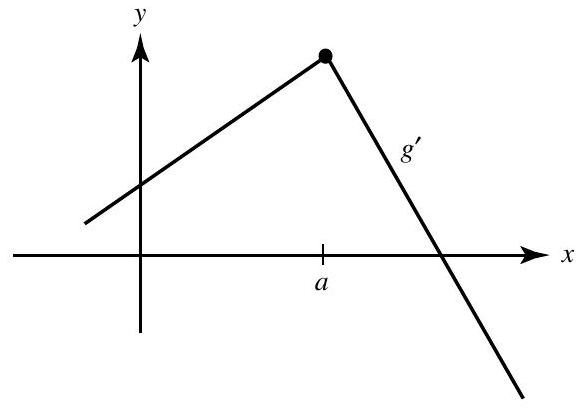
\includegraphics[width=0.40\linewidth]{calculus/images/a21d1d4b-31f6-4d46-a574-ed3f0f000705-09_409_585_937_1041.jpg}
\end{center}
\statementbox{%
\begin{enumerate}
\renewcommand{\labelenumi}{\Roman{enumi}.}
  \item $g$ is continuous.
  \item $g$ is differentiable.
  \item $g$ is increasing.
\end{enumerate}%
}
\begin{choices}
  \choice I only
  \choice III only
  \choice I and III only
  \choice II and III only
  \CorrectChoice I, II, and III
\end{choices}
\begin{solution}
Since $g^{\prime}(a)$ exists, $g$ is differentiable and thus continuous; $g^{\prime}(a)>0$.
\end{solution}

\question
A function $f$ has the derivative shown. Which of the following statements must be false?
\begin{center}
  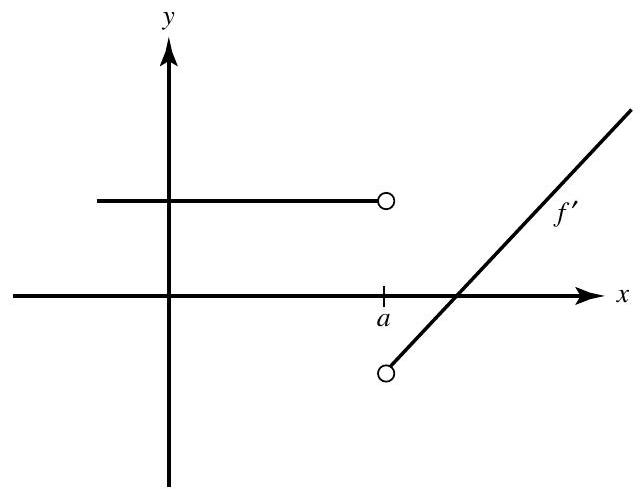
\includegraphics[width=0.40\linewidth]{calculus/images/a21d1d4b-31f6-4d46-a574-ed3f0f000705-09_497_642_1535_1008.jpg}
\end{center}
\begin{choices}
  \choice $f$ is continuous at $x=a$.
  \choice $f(a)=0$.
  \CorrectChoice $f$ has a vertical asymptote at $x=a$.
  \choice $f$ has a jump discontinuity at $x=a$.
  \choice $f$ has a removable discontinuity at $x=a$.
\end{choices}
\begin{solution}
Near a vertical asymptote the slopes must approach $\pm \infty$.
\end{solution}



\newpage



\question
The function $f$ whose graph is shown has $f^{\prime}=0$ at $x=$
\begin{center}
  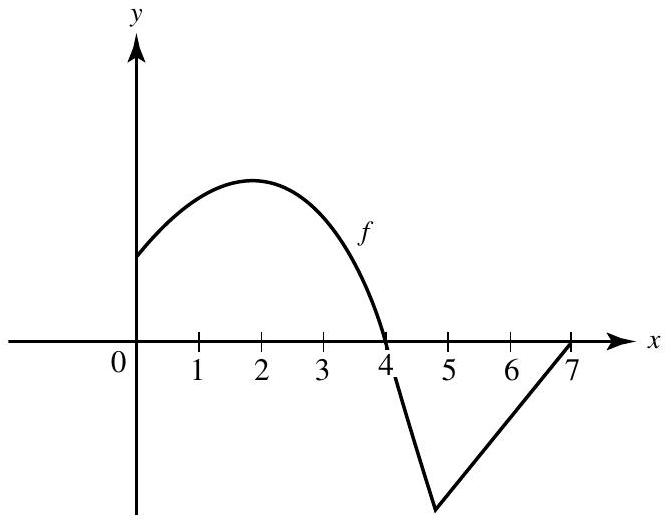
\includegraphics[width=0.40\linewidth]{calculus/images/a21d1d4b-31f6-4d46-a574-ed3f0f000705-09_522_671_2055_983.jpg}
\end{center}
\begin{choices}
  \CorrectChoice $2$ only
  \choice $2$ and $5$
  \choice $4$ and $7$
  \choice $2$, $4$, and $7$
  \choice $2$, $4$, $5$, and $7$
\end{choices}
\begin{solution}
There is only one horizontal tangent.
\end{solution}

\question
A differentiable function $f$ has the values shown. Estimate $f^{\prime}(1.5)$.


\begin{center}
\begin{tabular}{c|c|c|c|c}
$x$ & 1.0 & 1.2 & 1.4 & 1.6 \\
\hline
$f(x)$ & 8 & 10 & 14 & 22 \\
\end{tabular}
\end{center}
\begin{choices}
  \choice $8$
  \choice $12$
  \choice $18$
  \CorrectChoice $40$
  \choice $80$
\end{choices}
\begin{solution}
Use the symmetric difference quotient; then
\[
f^{\prime}(1.5) \approx \dfrac{f(1.6)-f(1.4)}{1.6-1.4}=\dfrac{8}{0.2}
\]
\end{solution}




\newpage




\question
Water is poured into a conical reservoir at a constant rate. If $h(t)$ is the rate of change of the depth of the water, then $h$ is
\begin{center}
  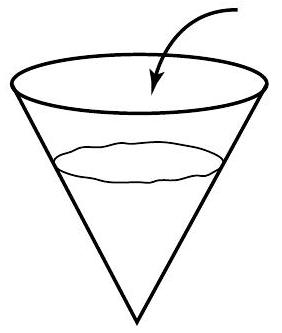
\includegraphics[width=0.40\linewidth]{calculus/images/a21d1d4b-31f6-4d46-a574-ed3f0f000705-10_333_282_695_1651.jpg}
\end{center}
\begin{choices}
  \choice constant
  \choice linear and increasing
  \choice linear and decreasing
  \choice nonlinear and increasing
  \CorrectChoice nonlinear and decreasing
\end{choices}
\begin{solution}
Since the water level rises more slowly as the cone fills, the rate of depth change is decreasing, as in (C) and (E). However, at every instant the portion of the cone containing water is similar to the entire cone; the volume is proportional to the cube of the depth of the water. The rate of change of depth (the derivative) is therefore not linear, as in (C).
\end{solution}



\newpage




\begin{EnvFullwidth}
\textit{Use the figure to answer Questions~\ref{calc03:figf-first}--\ref{calc03:figf-last}. The graph of $f$ consists of two line segments and a semicircle.}
\begin{center}
  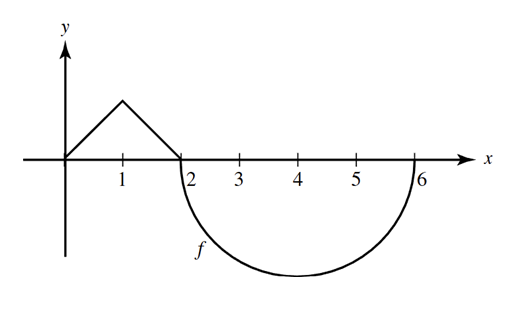
\includegraphics[width=0.40\linewidth]{calculus/images/more01.png}
\end{center}
\end{EnvFullwidth}
\question\label{calc03:figf-first}
$f^{\prime}(x)=0$ for $x=$
\begin{choices}
  \choice $1$ only
  \choice $2$ only
  \CorrectChoice $4$ only
  \choice $1$ and $4$
  \choice $2$ and $6$
\end{choices}
\begin{solution}
The only horizontal tangent is at $x=4$. Note that $f^{\prime}(1)$ does not exist.
\end{solution}

\question
$f^{\prime}(x)$ does not exist for $x=$
\begin{choices}
  \choice $1$ only
  \choice $2$ only
  \choice $1$ and $2$
  \choice $2$ and $6$
  \CorrectChoice $1$, $2$, and $6$
\end{choices}
\begin{solution}
The graph has corners at $x=1$ and $x=2$; the tangent line is vertical at $x=6$.
\end{solution}

\question\label{calc03:figf-last}
$f^{\prime}(5)=$
\begin{choices}
  \choice $\dfrac{1}{2}$
  \CorrectChoice $\dfrac{1}{\sqrt{3}}$
  \choice $1$
  \choice $2$
  \choice $\sqrt{3}$
\end{choices}
\begin{solution}
Consider triangle $A B C$ : $A B=1$; radius $A C=2$; thus, $B C=\sqrt{3}$ and $A C$ has $m=-\sqrt{3}$. The tangent line is perpendicular to the radius.\\
\begin{center}
  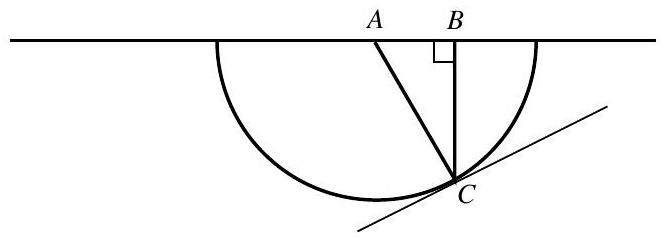
\includegraphics[width=0.40\linewidth]{calculus/images/a21d1d4b-31f6-4d46-a574-ed3f0f000705-21_245_666_1994_749.jpg}
\end{center}
\end{solution}


\newpage


\question
At how many points on the interval $[-5,5]$ is a tangent to $y=x+\cos x$ parallel to the secant line?
\begin{choices}
  \choice none
  \choice $1$
  \choice $2$
  \CorrectChoice $3$
  \choice more than $3$
\end{choices}
\begin{solution}
The graph of $y=x+\cos x$ is shown in window $[-5,5] \times[-6,6]$. The average rate of change is represented by the slope of secant segment $\overline{A B}$. There appear to be 3 points at which tangent lines are parallel to $\overline{A B}$.\\
\begin{center}
  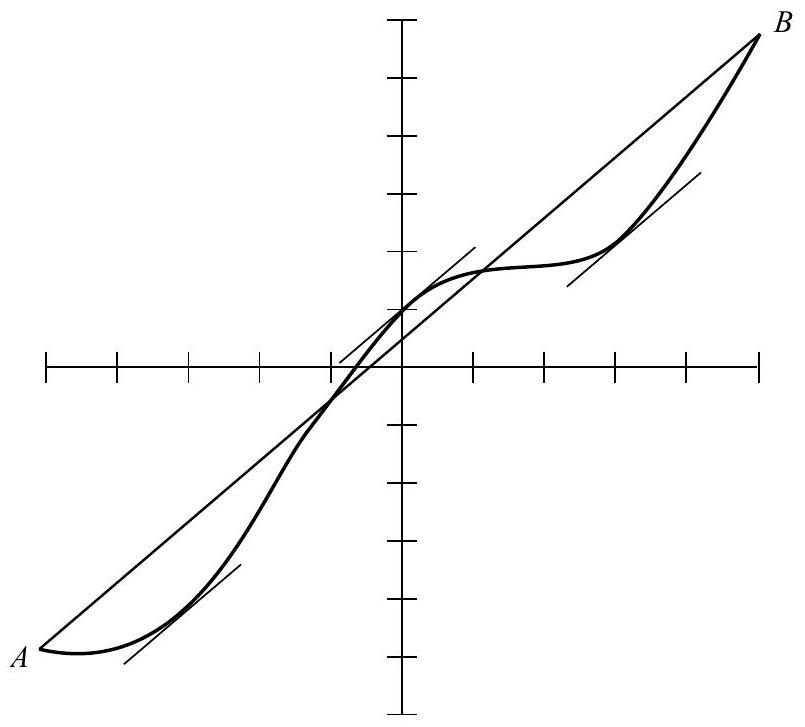
\includegraphics[width=0.40\linewidth]{calculus/images/a21d1d4b-31f6-4d46-a574-ed3f0f000705-22_727_805_487_1060.jpg}
\end{center}
\end{solution}

\question\label{calc03:est-fprime}
From the values of $f$ shown, estimate $f^{\prime}(2)$.

\begin{center}
\begin{tabular}{c|c|c|c|c|c}
$x$ & 1.92 & 1.94 & 1.96 & 1.98 & 2.00 \\
\hline
$f(x)$ & 6.00 & 5.00 & 4.40 & 4.10 & 4.00 \\
\hline
\end{tabular}
\end{center}
\begin{choices}
  \choice $-0.10$
  \choice $-0.20$
  \CorrectChoice $-5$
  \choice $-10$
  \choice $-25$
\end{choices}
\begin{solution}
$f^{\prime}(2) \simeq \dfrac{f(2)-f(1.98)}{2-1.98}=\dfrac{4.00-4.10}{0.02}$
\end{solution}




\newpage



\question
Using the values shown in the table for Question~\ref{calc03:est-fprime}, estimate $\left(f^{-1}\right)^{\prime}(4)$.
\begin{choices}
  \CorrectChoice $-0.2$
  \choice $-0.1$
  \choice $-5$
  \choice $-10$
  \choice $-25$
\end{choices}
\begin{solution}
Since an estimate of the answer for Question~\ref{calc03:est-fprime} is $f^{\prime}(2) \approx-5$, then $\left(f^{-1}\right)^{\prime}(4)=\dfrac{1}{f^{\prime}(2)} \approx \dfrac{1}{-5}=-0.2$.
\end{solution}

\question
The "left half" of the parabola defined by $y=x^{2}-8 x+10$ for $x \leq 4$ is a one-to-one function; therefore its inverse is also a function. Call that inverse $g$. Find $g^{\prime}(3)$.
\begin{choices}
  \choice $-\dfrac{1}{2}$
  \CorrectChoice $-\dfrac{1}{6}$
  \choice $\dfrac{1}{6}$
  \choice $\dfrac{1}{2}$
  \choice $\dfrac{11}{2}$
\end{choices}
\begin{solution}
When $x=3$ on $g^{-1}, y=3$ on the original half-parabola. $3=x^{2}-8 x+10$ at $x=1$ (and at $x=7$, but that value is not in the given domain).\\
$g^{\prime}(3)=\dfrac{1}{y^{\prime}(1)}=\left.\dfrac{1}{2 x-8}\right|_{x=1}=-\dfrac{1}{6}$.
\end{solution}

\question
The table below shows some points on a function $f$ that is both continuous and differentiable on the closed interval [2,10].

\begin{center}
\begin{tabular}{l|c|c|c|c|c}
$x$ & 2 & 4 & 6 & 8 & 10 \\
\hline
$f(x)$ & 30 & 25 & 20 & 25 & 30 \\
\end{tabular}
\end{center}

Which must be true?
\begin{choices}
  \choice $f(x)>0$ for $2<x<10$
  \choice $f^{\prime}(6)=0$
  \choice $f^{\prime}(8)>0$
  \choice The maximum value of $f$ on the interval $[2,10]$ is $30$ .
  \CorrectChoice For some value of $x$ on the interval $[2,10] f^{\prime}(x)=0$.
\end{choices}
\begin{solution}
$f$ satisfies Rolle's Theorem on $[2,10]$.
\end{solution}




\newpage




\question
If $f$ is differentiable and difference quotients overestimate the slope of $f$ at $x=a$ for all $h>0$, which must be true?
\begin{choices}
  \choice $f^{\prime}(a)>0$
  \choice $f^{\prime}(a)<0$
  \CorrectChoice $f^{\prime \prime}(a)>0$
  \choice $f^{\prime \prime}(a)<0$
  \choice none of these
\end{choices}
\begin{solution}
The diagrams show secant lines (whose slope is the difference quotient) with greater slopes than the tangent line. In both cases, $f$ is concave upward.\\
\begin{center}
  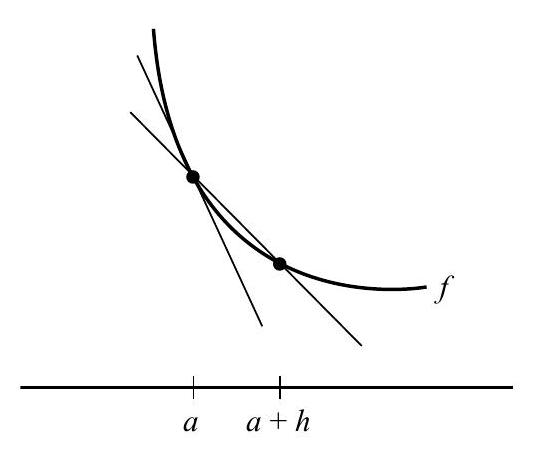
\includegraphics[width=0.40\linewidth]{calculus/images/a21d1d4b-31f6-4d46-a574-ed3f0f000705-22_449_536_2050_865.jpg}
\end{center}
\begin{center}
  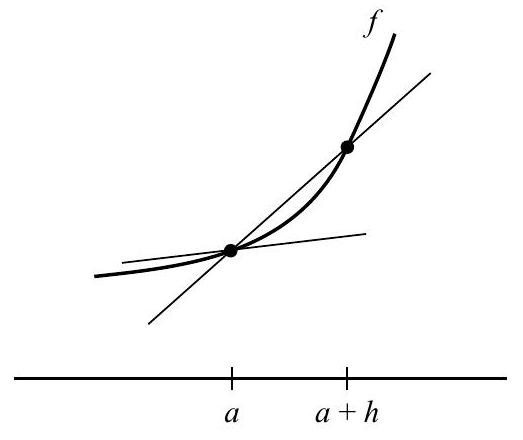
\includegraphics[width=0.40\linewidth]{calculus/images/a21d1d4b-31f6-4d46-a574-ed3f0f000705-22_440_523_2059_1516.jpg}
\end{center}
\end{solution}

\question
If $f(u)=\sin u$ and $u=g(x)=x^{2}-9$, then $(f \circ g)^{\prime}(3)$ equals
\begin{choices}
  \choice $0$
  \choice $1$
  \CorrectChoice $6$
  \choice $9$
  \choice none of these
\end{choices}
\begin{solution}
$(f \circ g)^{\prime}$ at $x=3$ equals $f^{\prime}(g(3)) \cdot g^{\prime}(3)$ equals $\cos u$ (at $u=0$ ) times $2 x$ (at $x=3$ ) $=1 \cdot 6=6$.
\end{solution}





\newpage



\question
If $f(x)=\dfrac{x}{(x-1)^{2}}$, then the set of $x$ 's for which $f^{\prime}(x)$ exists is
\begin{choices}
  \choice all reals
  \choice all reals except $x=1$ and $x=-1$
  \choice all reals except $x=-1$
  \choice all reals except $x=\dfrac{1}{3}$ and $x=-1$
  \CorrectChoice all reals except $x=1$
\end{choices}
\begin{solution}
Here $f^{\prime}(x)$ equals $\dfrac{-x-1}{(x-1)^{2}}$.
\end{solution}

\question
If $y=\sqrt{x^{2}+1}$, then the derivative of $y^{2}$ with respect to $x^{2}$ is
\begin{choices}
  \CorrectChoice $1$
  \choice $\dfrac{x^{2}+1}{2 x}$
  \choice $\dfrac{x}{2\left(x^{2}+1\right)}$
  \choice $\dfrac{2}{x}$
  \choice $\dfrac{x^{2}}{x^{2}+1}$
\end{choices}
\begin{solution}
$\dfrac{d y^{2}}{d x^{2}}=\dfrac{\dfrac{d y^{2}}{d x}}{\dfrac{d x^{2}}{d x}}$. Since $y^{2}=x^{2}+1, \dfrac{d y^{2}}{d x^{2}}=\dfrac{2 x}{2 x}$.
\end{solution}


\question
If $y=x^{2}+x$, then the derivative of $y$ with respect to $\dfrac{1}{1-x}$ is
\begin{choices}
  \CorrectChoice $(2 x+1)(x-1)^{2}$
  \choice $\dfrac{2 x+1}{(1-x)^{2}}$
  \choice $2 x+1$
  \choice $\dfrac{3-x}{(1-x)^{3}}$
  \choice none of these
\end{choices}
\begin{solution}
$\dfrac{d y}{d\left(\dfrac{1}{1-x}\right)}=\dfrac{\dfrac{d y}{d x}}{\dfrac{d\left(\dfrac{1}{1-x}\right)}{d x}}=\dfrac{2 x+1}{\dfrac{1}{(1-x)^{2}}}$.
\end{solution}





\newpage



\question
If $f(x)=\dfrac{1}{x^{2}+1}$ and $g(x)=\sqrt{x}$, then the derivative of $f(g(x))$ is
\begin{choices}
  \choice $\dfrac{-\sqrt{x}}{\left(x^{2}+1\right)^{2}}$
  \CorrectChoice $-(x+1)^{-2}$
  \choice $\dfrac{-2 x}{\left(x^{2}+1\right)^{2}}$
  \choice $\dfrac{1}{(x+1)^{2}}$
  \choice $\dfrac{1}{2 \sqrt{x}(x+1)}$
\end{choices}
\begin{solution}
Note that $f(g(x))=\dfrac{1}{x+1}$.
\end{solution}

\question
If $f(a)=f(b)=0$ and $f(x)$ is continuous on $[a, b]$, then
\begin{choices}
  \choice $f(x)$ must be identically zero
  \CorrectChoice $f^{\prime}(x)$ may be different from zero for all $x$ on $[a, b]$
  \choice there exists at least one number $c, a<c<b$, such that $f^{\prime}(c)=0$
  \choice $f^{\prime}(x)$ must exist for every $x$ on $(a, b)$
  \choice none of the preceding is true
\end{choices}
\begin{solution}
Sketch the graph of $f(x)=1-|x|$; note that $f(-1)=f(1)=0$ and that $f$ is continuous on $[-1,1]$. Only (B) holds.
\end{solution}

\question
Suppose $y=f(x)=2 x^{3}-3 x$. If $h(x)$ is the inverse function of $f$, then $h^{\prime}(-1)=$
\begin{choices}
  \choice $-1$
  \choice $\dfrac{1}{5}$
  \CorrectChoice $\dfrac{1}{3}$
  \choice $1$
  \choice $3$
\end{choices}
\begin{solution}
Since $f^{\prime}(x)=6 x^{2}-3$, therefore $h^{\prime}(x)=\dfrac{1}{6 x^{2}-3}$; also, $f(x)$, or $2 x^{3}-3 x$, equals -1 , by observation, for $x=1$. So $h^{\prime}(-1)$ or $\dfrac{1}{6 x^{2}-3}($ when $x=1)$ equals $\dfrac{1}{6-3}=\dfrac{1}{3}$.
\end{solution}





\newpage



\question
Suppose $f(1)=2, f^{\prime}(1)=3$, and $f^{\prime}(2)=4$. Then $\left(f^{-1}\right)^{\prime}(2)$
\begin{choices}
  \choice equals $-\dfrac{1}{3}$
  \choice equals $-\dfrac{1}{4}$
  \choice equals $\dfrac{1}{4}$
  \CorrectChoice equals $\dfrac{1}{3}$
  \choice cannot be determined
\end{choices}
\begin{solution}
$\left(f^{-1}\right)^{\prime}(2)=\dfrac{1}{f^{\prime}(1)}=\dfrac{1}{3}$.
\end{solution}

\question
If $f(x)=x^{3}-3 x^{2}+8 x+5$ and $g(x)=f^{-1}(x)$, then $g^{\prime}(5)=$
\begin{choices}
  \choice $8$
  \CorrectChoice $\dfrac{1}{8}$
  \choice $1$
  \choice $\dfrac{1}{53}$
  \choice $53$
\end{choices}
\begin{solution}
Since $f(0)=5, g^{\prime}(5)=\dfrac{1}{f^{\prime}(0)}=\left.\dfrac{1}{3 x^{2}-6 x+8}\right|_{x=0}=\dfrac{1}{8}$.
\end{solution}

\question
Suppose $\lim\limits_{x \to 0} \dfrac{g(x)-g(0)}{x}=1$. It follows necessarily that
\begin{choices}
  \choice $g$ is not defined at $x=0$
  \choice $g$ is not continuous at $x=0$
  \choice the limit of $g(x)$ as $x$ approaches $0$ equals $1$
  \CorrectChoice $g^{\prime}(0)=1$
  \choice $g^{\prime}(1)=0$
\end{choices}
\begin{solution}
The given limit is the derivative of $g(x)$ at $x=0$.
\end{solution}





\newpage



\begin{EnvFullwidth}
\textit{Use this graph of $y=f(x)$ for Questions~\ref{calc03:graphy-first}--\ref{calc03:graphy-last}.}
\begin{center}
  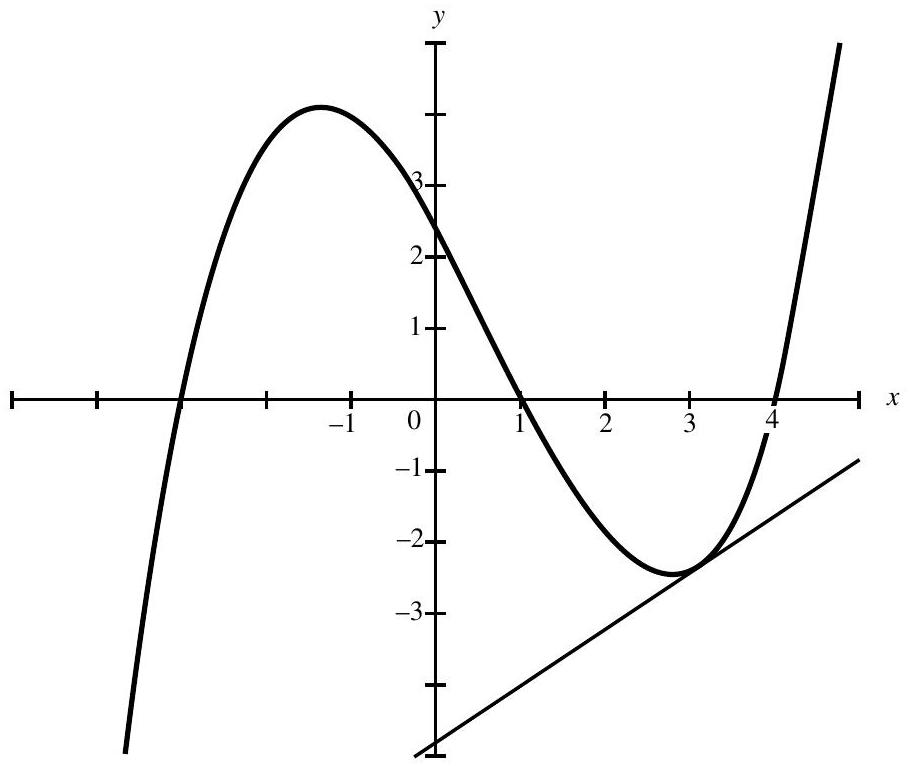
\includegraphics[width=0.40\linewidth]{calculus/images/a21d1d4b-31f6-4d46-a574-ed3f0f000705-13_766_910_364_533.jpg}
\end{center}
\end{EnvFullwidth}

\question\label{calc03:graphy-first}
$f^{\prime}(3)$ is most closely approximated by
\begin{choices}
  \choice $0.3$
  \CorrectChoice $0.8$
  \choice $1.5$
  \choice $1.8$
  \choice $2$
\end{choices}
\begin{solution}
The tangent line appears to contain $(3,-2.6)$ and $(4,-1.8)$.
\end{solution}

\question\label{calc03:graphy-last}
The rate of change of $f(x)$ is least at $x \simeq$
\begin{choices}
  \choice $-3$
  \choice $-1.3$
  \choice $0$
  \CorrectChoice $0.7$
  \choice $2.7$
\end{choices}
\begin{solution}
$f^{\prime}(x)$ is least at the point of inflection of the curve, at about 0.7 .
\end{solution}




\newpage




\begin{EnvFullwidth}
\textit{Use the following definition of the symmetric difference quotient for $f^{\prime}\left(x_{0}\right)$ for Questions~\ref{calc03:symdiff-first}--\ref{calc03:symdiff-last}. For small values of $h$,}
\[
f^{\prime}\left(x_{0}\right)=\dfrac{f\left(x_{0}+h\right)-f\left(x_{0}-h\right)}{2 h} .
\]
\end{EnvFullwidth}

\question\label{calc03:symdiff-first}
For $f(x)=5^{x}$, what is the estimate of $f^{\prime}(2)$ obtained 
by using the symmetric difference quotient with $h=0.03$?
\begin{choices}
  \choice $25.029$
  \choice $40.236$
  \CorrectChoice $40.252$
  \choice $41.223$
  \choice $80.503$
\end{choices}
\begin{solution}
$\dfrac{5^{2.03}-5^{1.97}}{2.03-1.97} \approx 40.25158$
\end{solution}

\question
To how many places is the symmetric difference quotient accurate when it is used to approximate $f^{\prime}(0)$ for $f(x)=4^{x}$ and $h=0.08$ ?
\begin{choices}
  \choice $1$
  \CorrectChoice $2$
  \choice $3$
  \choice $4$
  \choice more than $4$
\end{choices}
\begin{solution}
By calculator, $f^{\prime}(0)=1.386294805$ and $\dfrac{4^{0.08}-4^{-0.08}}{0.16}=1.3891 \ldots$.
\end{solution}

\question
To how many places is $f^{\prime}\left(x_{0}\right)$ accurate when it is used to approximate $f^{\prime}(0)$ for $f(x)=4^{x}$ and $h=0.001$ ?
\begin{choices}
  \choice $1$
  \choice $2$
  \choice $3$
  \choice $4$
  \CorrectChoice more than $4$
\end{choices}
\begin{solution}
Now $\dfrac{4^{0.001}-4^{-0.001}}{0.002}=1.386294805$.
\end{solution}





\newpage



\question\label{calc03:symdiff-last}
The value of $f^{\prime}(0)$ obtained using the symmetric difference quotient with $f(x)=|x|$ and $h=0.001$ is
\begin{choices}
  \choice $-1$
  \CorrectChoice $0$
  \choice $\pm 1$
  \choice $1$
  \choice indeterminate
\end{choices}
\begin{solution}
Note that any line determined by two points equidistant from the origin will necessarily be horizontal.\\
\begin{center}
  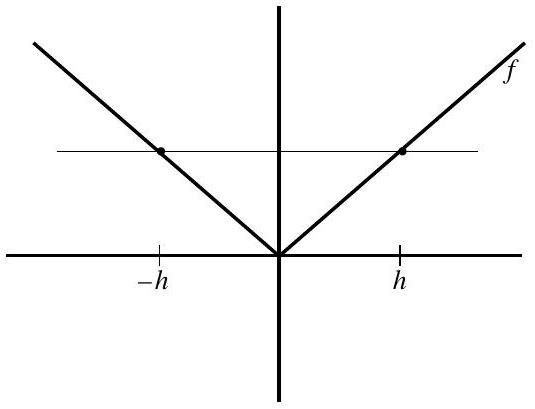
\includegraphics[width=0.40\linewidth]{calculus/images/a21d1d4b-31f6-4d46-a574-ed3f0f000705-24_409_535_392_1187.jpg}
\end{center}
\end{solution}

\question
If $\dfrac{d}{d x} f(x)=g(x)$ and $h(x)=\sin x$, then $\dfrac{d}{d x} f(h(x))$ equals
\begin{choices}
  \choice $g(\sin x)$
  \choice $\cos x \cdot g(x)$
  \choice $g^{\prime}(x)$
  \CorrectChoice $\cos x \cdot g(\sin x)$
  \choice $\sin x \cdot g(\sin x)$
\end{choices}
\begin{solution}
Note that $\dfrac{d}{d x} f(h(x))=f^{\prime}(h(x)) \cdot h^{\prime}(x)=g(h(x)) \cdot h^{\prime}(x)=g(\sin x) \cdot \cos x$.
\end{solution}

\question
Let $f(x)=3^{x}-x^{3}$. The tangent to the curve is parallel to the secant through $(0,1)$ and $(3,0)$ for $x=$
\begin{choices}
  \choice $0.984$ only
  \choice $1.244$ only
  \choice $2.727$ only
  \choice $0.984$ and $2.804$ only
  \CorrectChoice $1.244$ and $2.727$ only
\end{choices}
\begin{solution}
Since $f(x)=3^{x}-x^{3}$, then $f^{\prime}(x)=3^{x} \ln 3-3 x^{2}$. Furthermore, $f$ is continuous on $[0,3]$ and $f^{\prime}$ is differentiable on $(0,3)$, so the MVT applies. We therefore seek $c$ such that $f^{\prime}(c)=\dfrac{f(3)-f(0)}{3}=-\dfrac{1}{3}$. Solving $3^{x} \ln x-3 x^{2}=-\dfrac{1}{3}$ with a calculator, we find that $c$ may be either 1.244 or 2.727 . These values are the $x$-coordinates of points on the graph of $f(x)$ at which the tangents are parallel to the secant through points $(0,1)$ and $(3,0)$ on the curve.
\end{solution}





\newpage



\begin{EnvFullwidth}
\textit{Questions~\ref{calc03:graphf-first}--\ref{calc03:graphf-last} are based on the following graph of $f(x)$, sketched on $-6 \leqq x \leqq 7$. Assume the horizontal and vertical grid lines are equally spaced at unit intervals.}
\begin{center}
  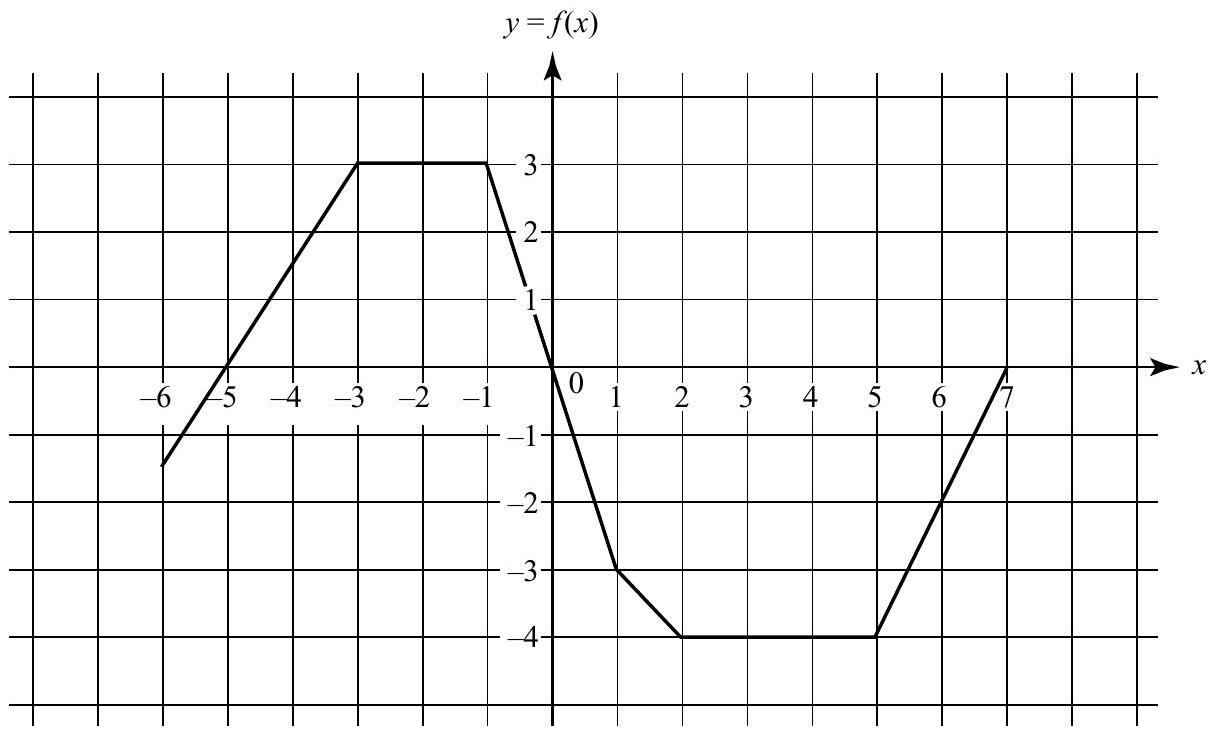
\includegraphics[width=0.70\linewidth]{calculus/images/a21d1d4b-31f6-4d46-a574-ed3f0f000705-14_741_1219_1257_760.jpg}
\end{center}
\end{EnvFullwidth}

\question\label{calc03:graphf-first}
On the interval $1<x<2, f(x)$ equals
\begin{choices}
  \CorrectChoice $-x-2$
  \choice $-x-3$
  \choice $-x-4$
  \choice $-x+2$
  \choice $x-2$
\end{choices}
\begin{solution}
The line segment passes through $(1,-3)$ and $(2,-4)$.
\textit{Use the graph of $f^{\prime}(x)$, shown below, for Questions~\ref{calc03:graphfp-first}--\ref{calc03:graphfp-last}.}
\begin{center}
  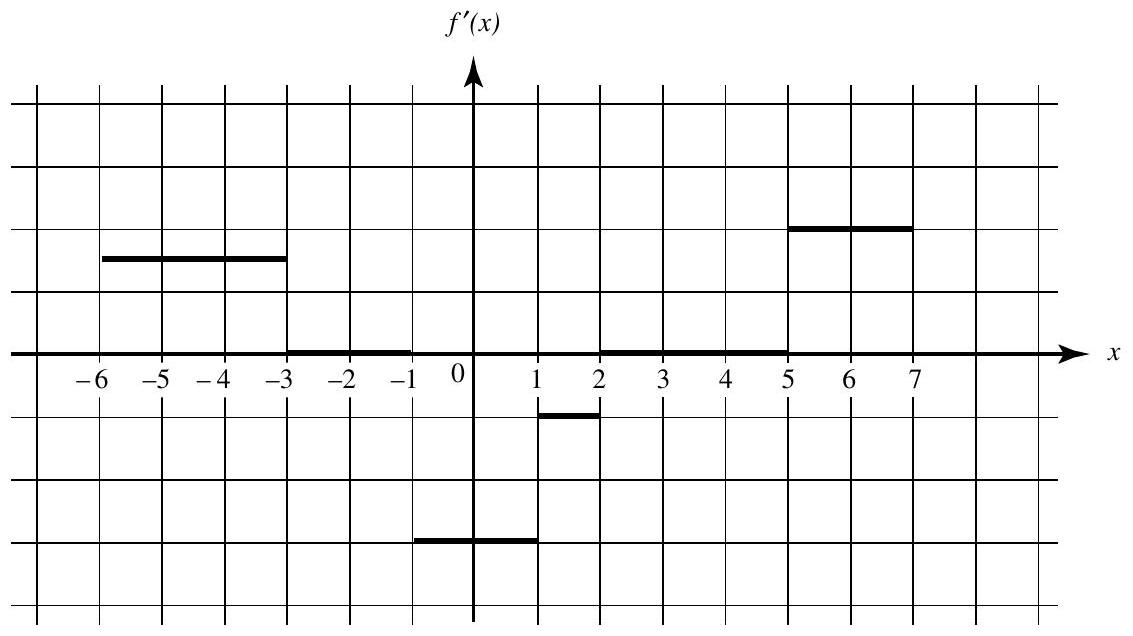
\includegraphics[width=0.70\linewidth]{calculus/images/a21d1d4b-31f6-4d46-a574-ed3f0f000705-24_636_1133_1438_904.jpg}
\end{center}
\end{solution}



\newpage




\question\label{calc03:graphfp-first}
Over which of the following intervals does $f^{\prime}(x)$ equal zero?
\statementbox{%
\begin{enumerate}
\renewcommand{\labelenumi}{\Roman{enumi}.}
  \item $(-6,-3)$
  \item $(-3,-1)$
  \item $(2,5)$
\end{enumerate}%
}
\begin{choices}
  \choice I only
  \choice II only
  \choice I and II only
  \choice I and III only
  \CorrectChoice II and III only
\end{choices}
\begin{solution}
(E) $f^{\prime}(x)=0$ when the slope of $f(x)$ is 0 ; that is, when the graph of $f$ is a horizontal segment.
\end{solution}

\question
How many points of discontinuity does $f^{\prime}(x)$ have on the interval $-6<x<7$ ?
\begin{choices}
  \choice none
  \choice $2$
  \choice $3$
  \choice $4$
  \CorrectChoice $5$
\end{choices}
\begin{solution}
(E) The graph of $f^{\prime}(x)$ jumps at each corner of the graph of $f(x)$, namely, at $x$ equal to $-3,-1,1,2$, and 5 .
\end{solution}

\question
For $-6<x<-3, f^{\prime}(x)$ equals
\begin{choices}
  \choice $-\dfrac{3}{2}$
  \choice $-1$
  \choice $1$
  \CorrectChoice $\dfrac{3}{2}$
  \choice $2$
\end{choices}
\begin{solution}
(D) On the interval $(-6,-3), f(x)=\dfrac{3}{2}(x+5)$.
\end{solution}




\newpage




\question\label{calc03:graphfp-last}\label{calc03:graphf-last}
Which of the following statements about the graph of $f^{\prime}(x)$ is false?
\begin{choices}
  \choice It consists of six horizontal segments.
  \CorrectChoice It has four jump discontinuities.
  \choice $f^{\prime}(x)$ is discontinuous at each $x$ in the set $\{-3,-1,1,2,5\}$.
  \choice $f^{\prime}(x)$ ranges from $-3$ to $2$ .
  \choice On the interval $-1<x<1, f^{\prime}(x)=-3$.
\end{choices}
\begin{solution}
(B) Verify that all choices but (B) are true. The graph of $f^{\prime}(x)$ has five (not four) jump discontinuities.
\end{solution}

\question
The table gives the values of a function $f$ that is differentiable on the interval $[0,1]$ :

\begin{center}
\begin{tabular}{c|c|c|c|c|c|c}
$x$ & 0.10 & 0.20 & 0.30 & 0.40 & 0.50 & 0.60 \\
\hline
$f(x)$ & 0.171 & 0.288 & 0.357 & 0.384 & 0.375 & 0.336 \\
\end{tabular}
\end{center}

According to this table, the best approximation of $f^{\prime}(0.10)$ is
\begin{choices}
  \choice $0.12$
  \choice $1.08$
  \CorrectChoice $1.17$
  \choice $1.77$
  \choice $2.88$
\end{choices}
\begin{solution}
(C) The best approximation to $f^{\prime}(0.10)$ is $\dfrac{f(0.20)-f(0.10)}{0.20-0.10}$.
\end{solution}




\newpage




\question
At how many points on the interval $[a, b]$ does the function graphed satisfy the Mean Value Theorem?
\begin{center}
  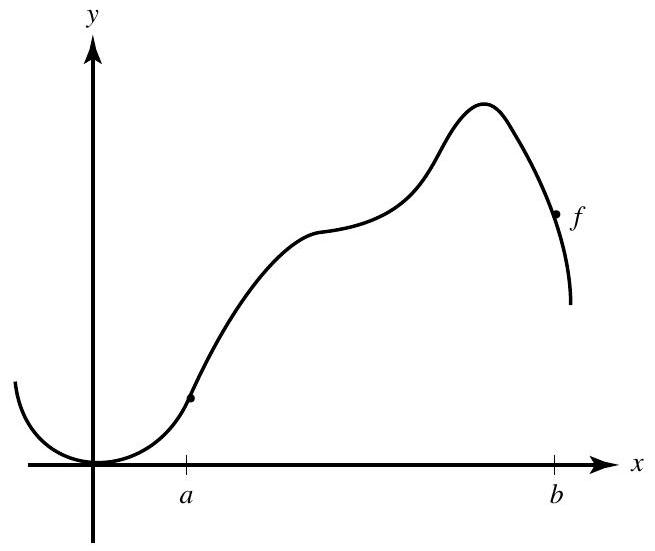
\includegraphics[width=0.40\linewidth]{calculus/images/a21d1d4b-31f6-4d46-a574-ed3f0f000705-15_551_655_1623_640.jpg}
\end{center}
\begin{choices}
  \choice none
  \choice $1$
  \choice $2$
  \CorrectChoice $3$
  \choice $4$
\end{choices}
\begin{solution}
(D) The average rate of change is represented by the slope of secant segment $\overline{A B}$. There appear to be 3 points at which the tangent lines are parallel to $\overline{A B}$.
\begin{center}
  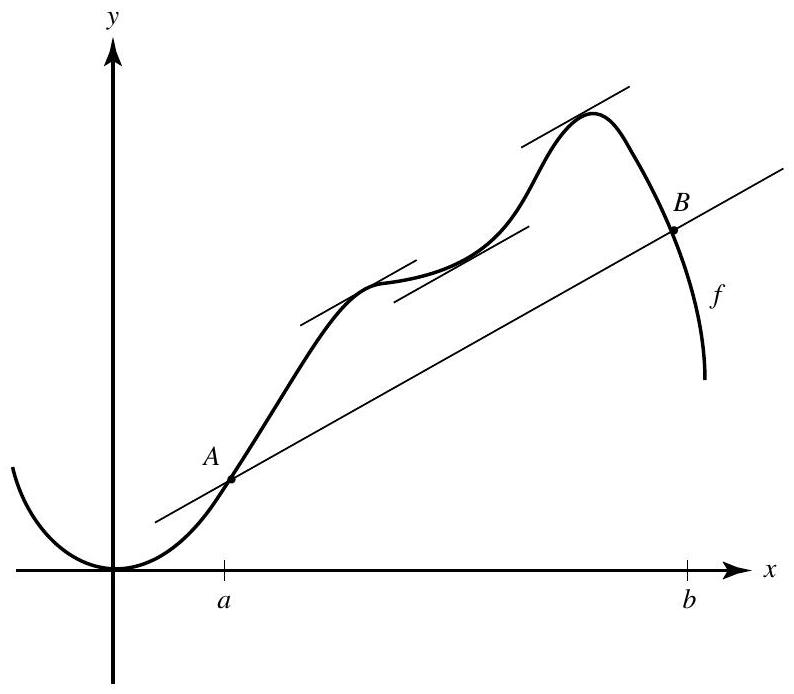
\includegraphics[width=0.40\linewidth]{calculus/images/a21d1d4b-31f6-4d46-a574-ed3f0f000705-25_694_794_559_668.jpg}
\end{center}
\end{solution}